\section{Thiết lập thực nghiệm}
\subsection{Bộ dữ liệu CICIDS2017}
Bộ dữ liệu CICIDS2017 do Viện An ninh mạng Canada (CIC) xây dựng, ghi lại lưu lượng mạng thực tế trong năm ngày làm việc với khoảng 2,83 triệu bản ghi luồng (flow). Mỗi luồng được trích xuất khoảng 80 đặc trưng thống kê bằng công cụ CICFlowMeter (thời lượng luồng, số gói, kích thước gói, cờ TCP, tốc độ byte/gói\dots). Dữ liệu bao gồm lưu lượng bình thường (BENIGN) và nhiều loại tấn công đa dạng: Brute Force (FTP/SSH), DoS/DDoS, PortScan, Web Attack, Infiltration, Botnet và Heartbleed.

Đặc điểm nổi bật của bộ dữ liệu là mất cân bằng nghiêm trọng (Hình~\ref{fig:balance}): lưu lượng bình thường chiếm áp đảo (khoảng 80\%), trong khi một số loại tấn công cực hiếm (ví dụ Heartbleed hay Infiltration chỉ có vài chục mẫu). Trong nghiên cứu này, chúng tôi quy về bài toán phân loại nhị phân (BENIGN so với ATTACK); dù mức mất cân bằng ở dạng nhị phân nhẹ hơn so với đa lớp, việc nhận diện chính xác các mẫu thuộc những loại tấn công hiếm vẫn là thách thức mà chiến lược lấy mẫu lai RUS-ENN hướng tới giải quyết. Dữ liệu được chia thành tập huấn luyện và tập kiểm thử độc lập; mọi bước cân bằng chỉ áp dụng trên tập huấn luyện để tránh rò rỉ dữ liệu.

\begin{figure}[!t]
\centering
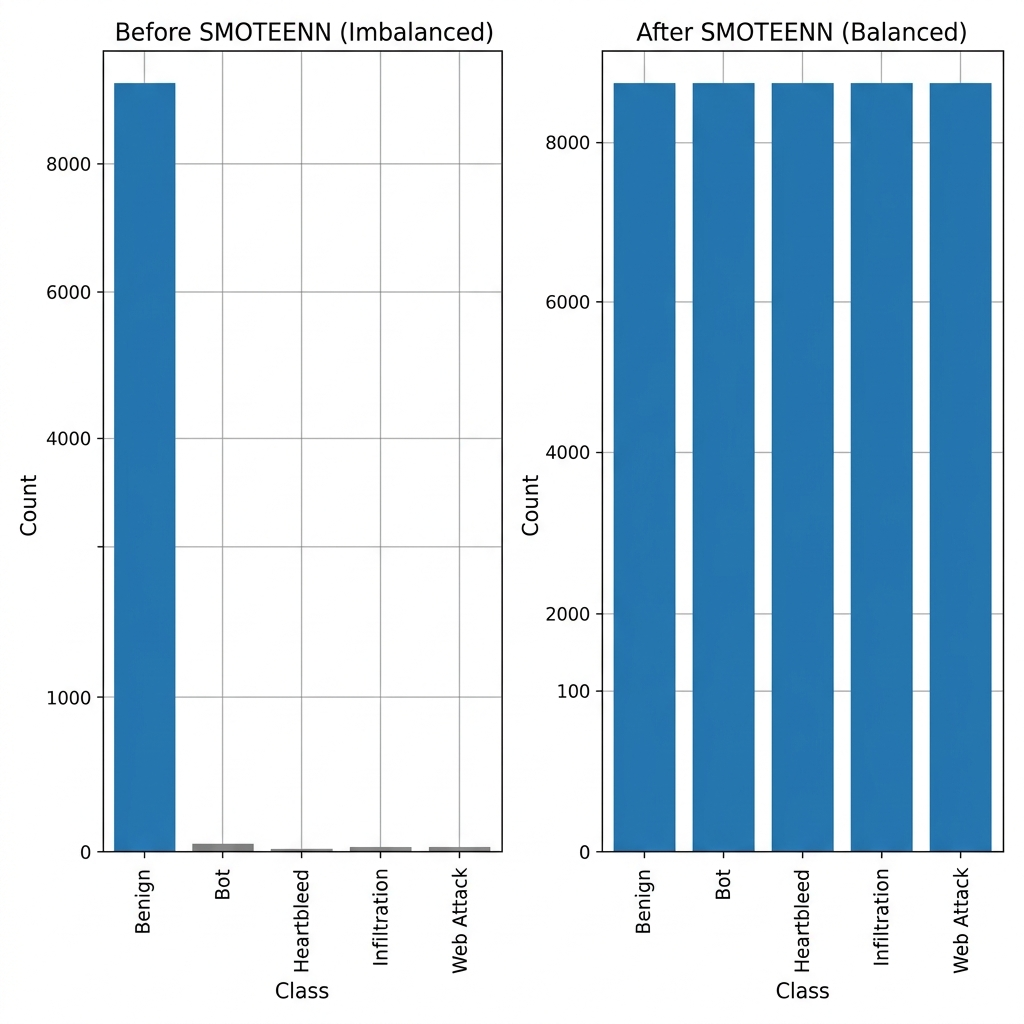
\includegraphics[width=\columnwidth]{figures/dataset_balance.png}
\caption{Phân bố lớp trên CICIDS2017 (nhị phân): lưu lượng bình thường áp đảo so với tấn công.}
\label{fig:balance}
\end{figure}

\subsection{Môi trường phần cứng và phần mềm}
Toàn bộ quá trình thực nghiệm (bao gồm huấn luyện mô hình Giáo viên và đánh giá tốc độ suy luận của mô hình Học sinh) đều được triển khai thống nhất trên nền tảng Google Colab Pro (Intel Xeon 2,20 GHz, 13 GB RAM, GPU NVIDIA Tesla T4 16 GB). Hệ thống được cài đặt trên ngôn ngữ Python 3.10.12, kết hợp với các thư viện nền tảng bao gồm Scikit-learn 1.2.2 và Imbalanced-learn 0.10.1. Để đảm bảo khả năng tái lập, mọi thực nghiệm dùng chung một hạt giống ngẫu nhiên cố định (\texttt{random\_state}=42). Cấu hình siêu tham số chính của các mô hình được tóm tắt trong Bảng~\ref{tab:hyperparams}.

\begin{table}[!t]
\centering
\caption{Cấu hình siêu tham số chính của các mô hình}
\label{tab:hyperparams}
\footnotesize
\begin{tabularx}{\columnwidth}{@{}lX@{}}
\toprule
\textbf{Mô hình} & \textbf{Siêu tham số} \\
\midrule
XGBoost       & n\_estimators=100; learning\_rate=0,1; max\_depth=6 \\
LightGBM      & n\_estimators=100; learning\_rate=0,1; max\_depth=6 \\
Random Forest & n\_estimators=100; max\_depth=20; min\_samples\_split=5; min\_samples\_leaf=2 \\
Meta-learner  & Hồi quy Logistic (class\_weight=balanced); số fold sinh đặc trưng OOF=5 \\
Student (DT)  & max\_depth=8; min\_samples\_split=10 \\
\bottomrule
\end{tabularx}
\end{table}

\subsection{Kịch bản thực nghiệm và đánh giá hiệu năng}
Chuỗi thực nghiệm gồm ba kịch bản chính:
\begin{enumerate}
    \item \textit{Tác động của tiền xử lý}: Đánh giá hiệu quả phương pháp lai RUS-ENN so với dữ liệu nguyên bản.
    \item \textit{Năng lực phát hiện}: So sánh độ chính xác của Teacher với các kiến trúc học máy phổ biến.
    \item \textit{Đánh giá tài nguyên tại biên}: So sánh kích thước mô hình và độ trễ suy luận trên CPU để làm rõ giá trị của chưng cất tri thức. Độ trễ được đo theo từng mẫu (batch\_size=1), mô phỏng kịch bản phát hiện tức thời; đây là cận trên của độ trễ thực tế khi suy luận theo lô.
\end{enumerate}

Do tập dữ liệu mất cân bằng nghiêm trọng, việc đánh giá chỉ dựa trên Accuracy sẽ không phản ánh đúng hiệu năng của mô hình. Do đó, chúng tôi sử dụng \textbf{F1-Score} làm tiêu chuẩn định lượng chính. Gọi $TP$, $FP$, $TN$, $FN$ lần lượt là số mẫu dương đúng, dương sai, âm đúng và âm sai. Các chỉ số được định nghĩa như sau:
\begin{equation}
\text{Precision} = \frac{TP}{TP+FP}, \qquad \text{Recall} = \frac{TP}{TP+FN},
\end{equation}
\begin{equation}
\text{F1} = 2\cdot\frac{\text{Precision}\cdot\text{Recall}}{\text{Precision}+\text{Recall}}, \qquad \text{FPR} = \frac{FP}{FP+TN}.
\end{equation}
Trong đó Precision phản ánh khả năng giảm cảnh báo giả, còn Recall (độ nhạy) phản ánh khả năng phát hiện tấn công thực tế. Ngoài F1 của lớp tấn công, chúng tôi còn báo cáo \emph{macro-F1} (trung bình F1 của hai lớp) để đánh giá công bằng trên dữ liệu mất cân bằng, cùng FPR để định lượng tỷ lệ cảnh báo giả. Để xác định liệu các chênh lệch nhỏ giữa các mô hình có ý nghĩa thống kê hay chỉ là nhiễu, chúng tôi sử dụng \emph{kiểm định McNemar} cho các cặp mô hình trên cùng tập kiểm thử và \emph{khoảng tin cậy 95\%} theo phương pháp bootstrap (1000 lần lấy mẫu lại) cho các chỉ số chính.
